\documentclass[12pt]{article}
\usepackage{array}
\usepackage{biblatex}
\usepackage{float}
\usepackage{graphicx}
\usepackage{hyperref}
\usepackage{indentfirst}
\usepackage[utf8]{inputenc}
\usepackage{listings}
\usepackage{xcolor}

\definecolor{codegreen}{rgb}{0,0.6,0}
\definecolor{codegray}{rgb}{0.5,0.5,0.5}
\definecolor{codepurple}{rgb}{0.58,0,0.82}
\definecolor{backcolour}{rgb}{0.95,0.95,0.92}

\lstdefinestyle{codestyle}{
    backgroundcolor=\color{backcolour},   
    commentstyle=\color{codegreen},
    keywordstyle=\color{magenta},
    numberstyle=\tiny\color{codegray},
    stringstyle=\color{codepurple},
    basicstyle=\ttfamily\footnotesize,
    breakatwhitespace=false,         
    breaklines=true,                 
    captionpos=b,                    
    keepspaces=true,                 
    numbers=left,                    
    numbersep=5pt,                  
    showspaces=false,                
    showstringspaces=false,
    showtabs=false,                  
    tabsize=2
}

\lstset{style=codestyle}


\addbibresource{main.bib}
\setlength{\parskip}{0.5em}

\title{
\includegraphics[keepaspectratio,width=0.5\paperwidth]{hku.png} \\ Refining Function Pointers’ Targets With\\ Class Hierarchy Tree Reconstruction and Object-Flow Analysis\\ \  \\Final Year Project Plan}
\author{Binrui Dong\\ (3035534816)\\ \ \\ Supervisor\\ Chenxiong Qian}
\date{\today}

\begin{document}

\maketitle

\newpage

\tableofcontents

\newpage

% \section{Introduction}

\section{Background}

This section will first introduce the background of Control Flow Integrity technique in subsection \ref{subsection:cfi}, then discuss the complications brought by function pointers in subsection \ref{subsection:fptr}, and introduce the state-of-the-art .

\subsection{Control Flow Integrity}
\label{subsection:cfi}

To date, many large modern software are written in C/C++ programming languages, from operating system kernels such as Linux and FreeBSD, to user space applications, including databases (e.g. MySQL, MongoDB), web browsers (e.g. Firefox, Chromium) and video game engines (e.g. Unreal Engine). C/C++ allows programmers to directly manipulate memory, which helps in building high performance software programs, however, it also leaves door open for potential security vulnerabilities \cite{BurowNathan2017CIPS}. Attackers may make use of oversights in the program (such as lack of input validation, array bounds checking, etc.) to corrupt memory, and divert the control-flow of the program away from its original legitimate region to malicious code.

\begin{figure}[b]
    \centering
    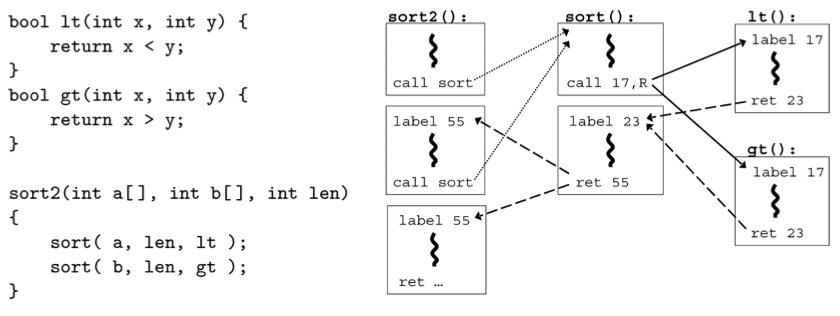
\includegraphics[keepaspectratio,width=0.55\paperwidth]{cfg.png}
    \caption{A piece of C code on the left, and its Control Flow Graph \cite{cfi2005}.}
    \label{fig:cfg}
\end{figure}

In response, \textbf{Control-Flow Integrity} (CFI) technique \cite{cfi2005} attempts to safeguard a program by restricting the control-flow of the program to its valid space \cite{nebelwelt}. The technique is composed of two phases, an ahead-of-time \textbf{analysis phase}, and a run-time \textbf{enforcement phase} \cite{BurowNathan2017CIPS}. During analysis phase, static analysis is performed on source code or binary of the program to compute its \textbf{Control-Flow Graph} (CFG), which basically represents the set of legitimate control-flow state transfers, such as function calls and returns. Then, during run-time enforcement phase, each control-flow state transfer is verified by checking if there is such an edge in CFG. If the transfer does not exist in the pre-computed CFG, then the control-flow integrity of the program must have been compromised, and actions can be taken as desired, for example, terminate the program execution, generate a memory dump for further investigation, send an alert to users and administrators, etc.

\subsection{CFG and Function Pointers}
\label{subsection:fptr}

\begin{figure}[h]
    \centering
    \begin{lstlisting}[language=c]
// Defines function pointer type
typedef int (*fptr_t)(int, int);

// Defines two functions of the type
int funcA(int a, int b) { return a + b; }
int funcB(int a, int b) { return a * b; }

// An indirect call happens here
int funcX(fptr_t p) { return p(2, 3); }

int main() { return funcX(&funcA); }
    \end{lstlisting}
    \caption{An example of function pointers and indirect function call}
    \label{fig:fptr}
\end{figure}

The construction of CFG is complicated by function pointers. For direct function calls like \texttt{memcpy(a, b, n);} and \texttt{fopen("file.txt", "r");}, it's known for sure that a function call to \texttt{memcpy} and \texttt{fopen} will happen at these places respectively. However, in case of an indirect function call through function pointers, the target function is not immediately known to static analysis. Figure \ref{fig:fptr} illustrates an example of such scenario. In the body of function \texttt{funcX()}, static analysis cannot immediately determine which target function is \texttt{p} referring to.

But function pointers are extensively used in practical software development. For example, in Linux kernel, in order to support \texttt{open()} system call on different file-systems, the kernel may store function pointers to the underlying implementations of such functionality for \texttt{ext4}, \texttt{xfs}, \texttt{btrfs}, etc., and dynamically invoke the corresponding underlying function during run-time depending on the file-system used \cite{mlta}. Function pointers are even essential in C++ run-time polymorphism. Each class, if contains virtual methods, maintains a virtual function table that stores function pointers to the actual concrete function implementations. During run-time, when invoking a virtual method of a class, the virtual function table of the class instance is looked up and an indirect call through the consulted function pointer takes place.

Previous approaches to deal with function pointers in constructing CFG includes rough type matching \cite{modular-cfi}. In the example of figure \ref{fig:fptr}, the type of function pointer \texttt{p} is \texttt{int(int, int)}, i.e., a function takes two \texttt{int} parameters and returns an \texttt{int} value. Then all functions with the same type are considered to be possible target functions. Hence, the indirect call \texttt{p(2, 3);} may transfer to both \texttt{funcA} and \texttt{funcB}, even though it can be seen that only \texttt{funcA} will be called and \texttt{funcB} will never be invoked.

As illustrated by the above example, this approach will inevitably yield a lot of false positive transfers, which in reality will never happen during a valid program execution. This negatively impacts the performance of CFI enforcement, since more edges need to be stored and to be checked. Moreover, this also weakens the effectiveness of CFI technique, as some invalid transfers could be regarded as valid and causing the malicious attack to remain unnoticed. A more precise approach to resolve target functions of function pointers is desirable.

\subsection{Multi-Layer Type Analysis}
\label{subsection:mlta}

The current state-of-the-art function pointer analysis technique is Multi-Layer Type Analysis proposed by Kangjie Lu and Hong Hu in their paper \cite{mlta} on the 26-th ACM Conference on Computer and Communications Security in 2019.

The technique attempts to improve the accuracy of resolving indirect call target functions by looking into the multi-layer type hierarchy information of the chain of \texttt{struct}s or \texttt{class}s in which the function pointer is stored.

\begin{figure}[t]
    \centering
    \begin{lstlisting}[language=c]
// Defines function pointer type
typedef int (*fptr_t)(int, int);

// Defines two functions of the type
int funcB(int a, int b) { return a + b; }
int funcC(int a, int b) { return a * b; }

// Defines three structs
struct A { fptr_t p; };
struct B { struct A a; };
struct C { struct A a; };

// Defines two instances of structs
struct B b = { .a = { .p = &funcB } };
struct C c = { .a = { .p = &funcC } };

int main() { return c.a.p(2, 3); }
    \end{lstlisting}
    \caption{Code example of Multi-Layer Type Analysis}
    \label{fig:mlta}
\end{figure}

In a simplified example illustrated in figure \ref{fig:mlta}, for the indirect call \texttt{c.a.p()} in \texttt{main()} function, Multi-Layer Type Analysis will notice that the function pointer \texttt{p} is stored in a \texttt{struct} of type \texttt{A}, which is in turn stored in a parent \texttt{struct} of type \texttt{C}. Then the scope of possible target functions for this indirect call is limited to those functions whose address are stored to pointers with the same multi-layer type hierarchy information, that is, function pointers that are also stored in a \texttt{struct} of type \texttt{A} in a parent \texttt{struct} of type \texttt{C}. In the example in figure \ref{fig:mlta}, the only function satisfying such condition is \texttt{funcC}, since its address is stored to a \texttt{struct} of type \texttt{A} in a parent \texttt{struct} of type \texttt{C} at line 15. Although funciton \texttt{funcB} also has the same function type (taking two \texttt{int} parameters and returns an \texttt{int} value), the address of \texttt{funcB} is never assigned to a \texttt{struct} of type \texttt{A} in a parent \texttt{struct} of type \texttt{C}.

This approach is based on the intuition that in practical software development, function pointers are often stored in multi-layer objects of objects \cite{mlta}, and this is indeed effective in field test. The authors evaluated their technique on three real-world system programs, Linux, FreeBSD and Firefox, and observed 86\% to 98\% reduction in the target functions reported for indirect calls \cite{mlta}.

\section{Objective}
This project aims to further refine the resolution of target functions of function pointers with object-flow analysis, which will be elaborated in the next section.

\section{Methodology}

This section will first introduce the technology stack the project will be built upon in subsection \ref{subsection:llvm}, then discuss the two methodologies used by the project, class hierarchy tree reconstruction, and object-flow analysis, in subsection \ref{subsection:class-tree} and subsection \ref{subsection:object-flow} respectively, and finally discuss evaluation of the work in subsection \ref{subsection:evaluation}.

\subsection{LLVM}
\label{subsection:llvm}

LLVM is a compiler and toolchain technologies framework \cite{llvm-website} composed of a collection of projects, most notably are

\begin{itemize}
    \item Clang, an optimizing C/C++/Objective-C compiler
    \item LLVM Core, a set of libraries offering architecture independent optimization and code generation support for different CPU architectures
\end{itemize}

who are designed to work closely with an architecture independent and programming language independent intermediate representation called LLVM IR, which is similar to assembly language, but is portable and preserves certain high-level language information, such as strong types and functions \cite{llvm-ir}.

\begin{figure}[t]
    \centering
    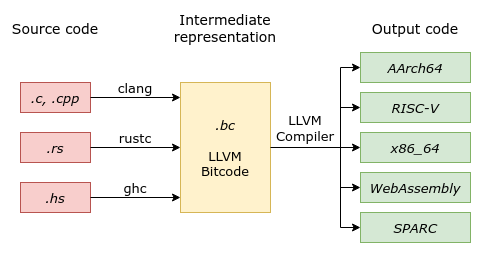
\includegraphics[keepaspectratio,width=0.6\paperwidth]{llvm-compiler.png}
    \caption{LLVM Compiling Pipeline \cite{llvm-pipeline}}
    \label{fig:llvm-compiler}
\end{figure}

Figure \ref{fig:llvm-compiler} shows the process of compiling a program from source code (e.g. a piece of C/C++ or Rust source code) to a binary executable that is runnable on a target architecture (e.g. x86) in LLVM. The compiler, Clang for C/C++ or \texttt{rustc} for Rust programs, will take source code as input, and generate LLVM IR stored in LLVM bitcode (\texttt{.bc}) file format. LLVM backend will then generate assembly code for target architecture from the LLVM bitcode.

\begin{figure}[H]
    \centering
    \begin{lstlisting}[language=c]
double square(double num) {
    return num * num;
}
    \end{lstlisting}
    \begin{lstlisting}[language=llvm]
define dso_local double @_Z6squared(double %0) local_unnamed_addr #0 {
  %2 = fmul double %0, %0
  ret double %2
}
    \end{lstlisting}
    \begin{lstlisting}[language={[x86masm]Assembler}]
square:
    sub     esp, 12
    movsd   xmm0, qword ptr [esp + 16]
    mulsd   xmm0, xmm0
    movsd   qword ptr [esp], xmm0
    fld     qword ptr [esp]
    add     esp, 12
    ret
    \end{lstlisting}
    \caption{C++ code, its LLVM IR, and its assembly code}
    \label{fig:llvm-ir}
\end{figure}

Figure \ref{fig:llvm-ir} illustrates an example of a C++ function being compiled to LLVM IR and x86 assembly code. Notice that function body, function name (\texttt{\_Z6squared} instead of \texttt{square} is because of C++ name mangling to support function overload) and both function types and variable types are fully preserved in LLVM IR. In x86 assembly code, however, these information are mostly lost.

The project will be implemented as a LLVM pass. A LLVM pass is a program that takes LLVM IR as input, and can perform analysis, optimizations and transformations on the LLVM IR code read \cite{llvm-pass}. In the scope of this project, the LLVM pass to be built will only need to perform read-only analysis on LLVM IR.

The software project to be analyzed will first need to be compiled to LLVM bitcode files. For example, a C++ source file \texttt{main.cpp} can be compiled to LLVM bitcode by \texttt{clang++ main.cpp -c -emit-llvm -o main.bc}. Then the LLVM pass will read those compiled LLVM bitcode files to performs function pointer targets analysis on those LLVM IR code.

Since LLVM IR preserves types and functions from program source code, this approach offers more information available to the analysis, in comparison to analyzing directly on the executable binary in target architecture machine code (e.g. x86).

\subsection{Class Hierarchy Tree Reconstruction}
\label{subsection:class-tree}

\begin{figure}[t]
    \centering
    \begin{lstlisting}[language=c++]
class Animal {
    public:
        virtual std::string Name() { return "Animal"; }
};

class Pet : public Animal {
    public:
        std::string Name() override { return "Pet"; }
};

class Dog : public Pet {
    public:
        std::string Name() override { return "Dog"; }
};
    \end{lstlisting}
    \caption{An example C++ class hierarchy}
    \label{fig:class-hierarchy}
\end{figure}

Class hierarchy tree reconstruction refers to recovering information of C++ class inheritance information from LLVM IR, in order to refine the scope of possible target functions of a class method invocation.

In figure \ref{fig:class-hierarchy}, the superclass \texttt{Animal} has a method \texttt{Name}. Class \texttt{Pet} inherits from class \texttt{Animal} and overrides method \texttt{Name}. Class \texttt{Dog} inherits from class \texttt{Pet} and overides method \texttt{Name} again.


When analyzing the function body of \texttt{funcA()} in figure \ref{fig:class-caller}, with class hierarchy tree information, it can be deduced that the possible target functions of \texttt{object->Name()} can only be either \texttt{Pet::Name()} or \texttt{Dog::Name()}, but not \texttt{Animal::Name()}, because \texttt{object} is of type \texttt{Pet}, and \texttt{Animal} is neither the class \texttt{Pet} itself nor its subclass, so \texttt{Animal::Name()} must not be a target function.

\begin{figure}[H]
    \centering
    \begin{lstlisting}[language=c++]
void funcA(Pet *object) {
    std::cout << object->Name() << std::endl;
}

void funcB() {
    Pet *object = new Dog;
    funcA(object);
    delete object;
}
    \end{lstlisting}
    \caption{Calling class methods}
    \label{fig:class-caller}
\end{figure}


\subsection{Object-Flow Analysis}
\label{subsection:object-flow}

Class hierarchy tree reconstruction can eliminate overridden superclass methods in target functions resolution, but it can be made more accurate, by analyzing not only the semantic type of an object as written in source code, but also what concrete types \textit{the instance} could possibly take.

In the example in figure \ref{fig:class-hierarchy} and figure \ref{fig:class-caller}, \texttt{funcA()} is only called in \texttt{funcB()}. In \texttt{funcB()}, although pointer \texttt{object} is declared with type of \texttt{Pet}, it is subsequently assigned with a \texttt{Dog} instance at line 6, and is passed as parameter to \texttt{funcA()}. In this example, the only type \texttt{object} can actually take in \texttt{funcA()} is \texttt{Dog}, and further refine the target functions set of method call \texttt{object->Name()} at line 2 in \texttt{funcA()} to only contain \texttt{Dog::Name()}.

Object-flow analysis keeps track of the set of possible concrete types that an object may take, in order to realize the intuition described above.

A possible approach to implement object-flow analysis is iterative search. Starting with an initial set of possible concrete types an object can take, it follows the logic flow of the program and detects if there is any value assignments to the object. There could be an instance of another concrete type assigned to the object. If this happens, then add the new concrete type to the set. Repeat the process, until the set is stabilized, i.e., no more type can be added to the set.

When analyzing a large code base, however, running time and memory consumption of the above method could be a concern. A big C++ project may contains thousands of compilation units and hundreds of thousands of functions and variables. It is hardly feasible to fit everything in memory during analysis. Some optimizations and trade-offs may need to be made, in order to make the object-flow analysis practical in real-world use scenario.

\subsection{Evaluation}
\label{subsection:evaluation}

After the LLVM pass is implemented, the analysis will be performed on real-world large scale C++ projects, such as Chromium, an open source web browser engine with around 12 million lines of C++ code as analyzed around August 2019 \cite{chromium-loc}.

The performance of the LLVM pass developed in the project, as well as the target functions resolution results produced, will be analyzed and compared to other previous approaches in resolution of target functions of function pointers, such as type matching \cite{modular-cfi} and multi-layer type analysis \cite{mlta} described in subsection \ref{subsection:mlta}.

\newpage
\section{Schedule}

\begin{table}[h]
    \centering
    \begin{tabular}{ | m{3cm} | m{7cm}| m{1.5cm} | } 
     \hline
     Time Point & Task & Status \\
     \hline
     \hline
     September 2021 & 
     Submission of first phase deliverable:
     \begin{itemize}
         \item Project Plan
         \item Project Web Page set-up
     \end{itemize} &
     Done
     \\[0.5cm]
     \hline
     October 2021 & 
     Research on previous work &
     Working
     \\[0.5cm]
     \hline
     November 2021 & 
     Preliminary system design &
     Pending
     \\[0.5cm]
     \hline
     January 2022 & 
     Submission of Intermediate Report &
     Pending
     \\[0.5cm]
     \hline
     February 2022 & 
     System implementation &
     Pending
     \\[0.5cm]
     \hline
     March 2022 & 
     Performance evaluation &
     Pending
     \\[0.5cm]
     \hline
     April 2022 & 
     Submission of Final Report &
     Pending
     \\[0.5cm]
     \hline
    \end{tabular}
    \caption{Project Schedule}
    \label{tab:schedule}
\end{table}

\newpage

\printbibliography

\end{document}
